\documentclass[]{article}
\usepackage[T1]{fontenc}
\usepackage[utf8]{inputenc}
\usepackage[french]{babel}
\usepackage[]{graphicx}
\usepackage[]{hyperref}

\title{Bilan de projet}
\author{
    Théo Delmas\\
    Lauric Teysseyre\\
    Pierre-Louis Renon\\
    Julien Wattier\\
    \\
    Université Paul Sabatier\\
    Master Informatique 1\\
   } 

\begin{document}
\maketitle
\newpage
\tableofcontents
\newpage

\begin{section}{Objectif du document}
 Ce document présente le bilan du projet.
\end{section}

{
\setlength{\parindent}{0pt} %Retire les alinéas
\begin{section}{Référentiel initial}
 \begin{subsection}{Produits initiaux}
     Le product breakdown initial ainsi que les méthodes de réalisation étaient les suivants :

     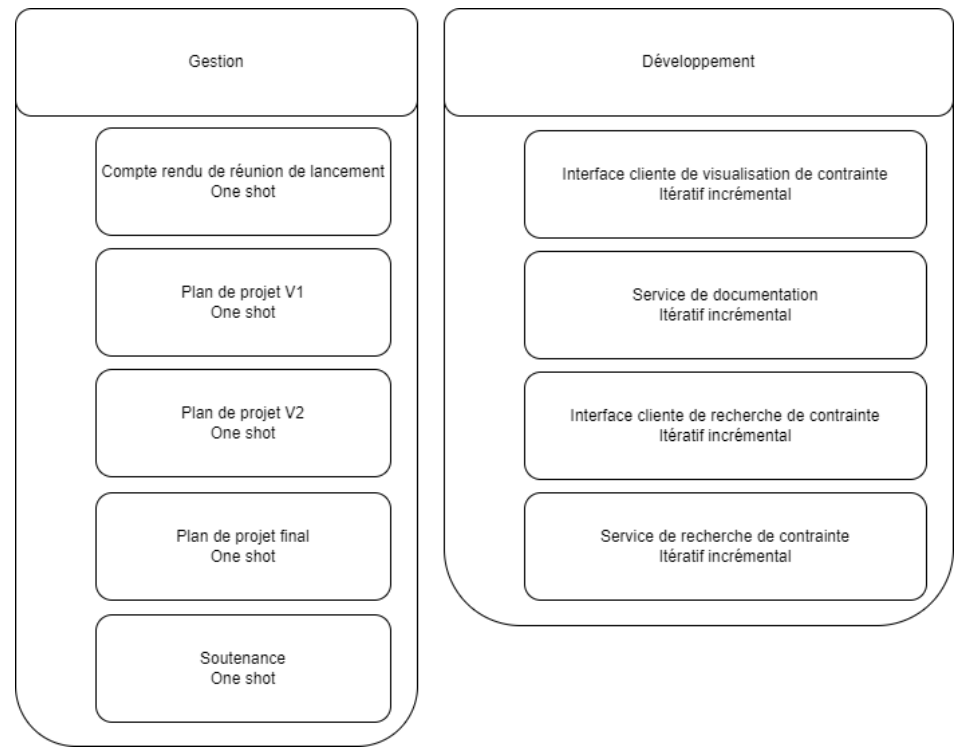
\includegraphics[scale=0.6]{IMG/PBS_initial}
 \end{subsection}
\end{section}

\begin{section}{État courant à la terminaison}
 \begin{subsection}{Produits réalisés}
     L’état des produit à la terminaison du projet sont exposés dans le schéma ci-dessous. Le code couleur indique leur état selon le code suivant :

     \begin{itemize}
         \item Vert : Le produit a été réalisé.
         \item Jaune : Le produit va être réalisé.
         \item Rouge : Le produit n’a pas été réalisé.
     \end{itemize}

     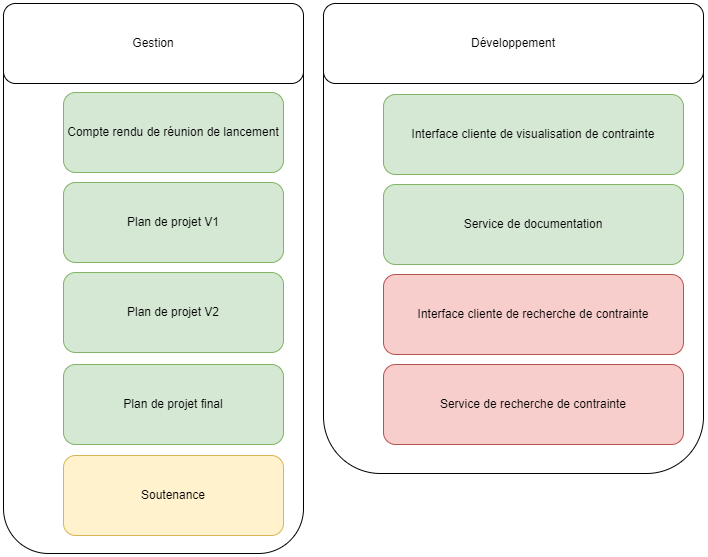
\includegraphics[scale=0.49]{IMG/PBS_final}

     La soutenance va être produit après la clôture du plan projet fixé au 14/03/2023.

     Concernant les produits liés au système de recherche de contrainte, il a été décidé début mars et avec accord du client qu’ils ne seraient pas produits faute de temps.
 \end{subsection}

 \begin{subsection}{Listes des événements}
    Le \href{Registre_des_faits_marquants.pdf}{registre des faits marquants} référence l'ensemble des événements ayant affecté le projet.
\end{subsection}

 \begin{subsection}{Listes des décisions}
     Conformément à la gestion des décision du plan de projet, le \href{Registre_des_décisions.pdf}{registre des décisions} référence l'ensemble des décisions ayant amendé le plan de projet.
 \end{subsection}

 \begin{subsection}{Listes des livrables de gestion}
    L'ensemble des livrables de gestion sont disponibles sur ce \href{https://github.com/Szyckaa/UE-PROJET-DOCS-GESTION}{dépot github}, en consultant les releases.
\end{subsection}

\newpage

\begin{subsection}{Listes des livrables de développement}
    L'ensemble des livrables de développement sont disponibles sur le \href{https://framagit.org/flopedt/FlOpEDT}{dépot framagit du projet}. Conformément à notre gestion des livrables, les livrables sont intégrés dans la \href{https://framagit.org/flopedt/FlOpEDT/-/tree/catalog}{branche catalog}. 
\end{subsection}
\end{section}

\begin{section}{Analyse du déroulement du projet}
    \begin{subsection}{Manque de contrôle}
        \begin{subsubsection}{Faute d'indicateur}
        
        \end{subsubsection}

        \begin{subsubsection}{Faute de processus}
        
        \end{subsubsection}
    \end{subsection}

    \begin{subsection}{Analyse de performance}
        Analyser le fichier calc, le critiquer (dire qu'en fait on ne cochait pas forcément au bon moment, que parfois les tâches étaient ajouté après avoir été faites)
    \end{subsection}

    \begin{subsection}{Un processus peu garant de la qualité}
        Définition de ready/done un peu légère
        Pas de test
    \end{subsection}

    \begin{subsection}{Un gestion du besoin initialement trop faible}
        Au début du projet l'équipe ne produisait pas de rapport de réunion qui mettent en relief les actions à effectuer pour le projet. De fait les tâches à effectuer n'étaient pas forcément mise à jour dans l'immédiat et certaines ont été temporairement oubliées. 
        
        Cela n'a que peu impacté le projet car les tâches oubliées n'étaient pas prioritaires mais cela aurait pu grandement impacter les artefacts produits en créant une différence entre ce qu'attendait le client et ce que produisait l'équipe.
    \end{subsection}

    \begin{subsection}{Une méthode de développement non optimale}
        L'équipe n'était pas suffisament rigoureuse dans la gestion des besoins et des actions a effectué. Pour rappel elle référencé uniquement les besoins dans un kanban et ajoutait sur chacun des tâches à réaliser.
    \end{subsection}

    \begin{subsection}{Des communications internes immédiates}
        L'équipe a essentiellement travaillé en distanciel depuis chez elle. Néamoins elle a dès le début décidé d'être systématiquement sur discord en vocal afin de partager immédiatement en cas de problème. Cela a permis d'éviter que les développeurs ne buttent trop longtemps sur des problèmes, mais également d'avoir un haut degré de partage de compétence.
    \end{subsection}
\end{section}

\begin{section}{Leçons apprises}
\end{section}

\begin{section}{Perspectives}

\end{section}

\begin{section}{Recommandations}
    \begin{subsection}{Migrer avant d'étendre}
        Pour rappel l'application est actuellement en train de migrer d'une application monolothique Django vers un front VueJS et un back Django dissociés. Notre travail consistait à étendre l'application en ajoutant un système. Au vu du contexte le client souhaitait que les nouveaux développements respectent la nouvelle philosophie de front et back dissociés. 
        
        Malheureusement cela a rendu nos développements compliqué en nous forçant à nous adapter à un code qui est voué à disparaître, notamment côté front. Nous pensons que la migration devrait être effectuée avant de réaliser des extensions.
    \end{subsection}

    \begin{subsection}{Documentation du code source}
        L'équipe qui maintient le projet devrait mettre en place une documentation assez généraliste qui décrit qu'est ce que chaque partie du projet réalise en ajoutant des markdowns dans les différents dossiers du projet.
    \end{subsection}
\end{section}

}
\end{document}